\chapter{Результаты анализа коллективной анизотропии}

\section{Результаты анализа экспериментальных данных HADES}

\section{Оценка вклада непотоковых корреляций в значения поправочного коэффициента разрешения $R_1$}

Для оценки систематики из-за непотоковых корреляций в полученных результатах $v_1$, был использован аналогичный метод, что и для разрешения плоскости симметрии. 
Для каждой плоскости симметрии, направленный поток может быть скорректирован на поправочный коэффициент разрешения рассчитанный с использованием различных комбинаций $Q_1$-векторов.
Сравнивая значения поправочного коэффициента, полученного при помощи различных комбинаций, можно оценить вклад непотоковых корреляций между $Q_1$-векторами.
Для проверки величины непотоковых корреляций между векторами частиц $u_1$ и вектором плоскости симметрии $Q_1$, можно сравнить значения $v_1$, полученные относительно различных плоскостей симметрии.
Таким образом, сравнивая направленный поток $v_1$, полученный относительно различных плоскостей симметрии и деленный на поправочный коэффициент разрешения, вычисленный с использованием различных комбинаций $Q_1$-векторов.

На рис.~\ref{fig:hades_w1w3} представлен направленный поток протонов $v_1$, рожденных в столкновении Au+Au при энергии $E_{kin}=$1.23$A$~ГэВ, как функция центральности столкновения, измеренный относительно различных $Q_1$-векторов. 
Коррекция на поправочный коэффициент разрешения выполнена с использованием различных комбинаций $Q_1$-векторов.
Слева представлены значения $v_1$ протонов измеренный относительно внутреннего подсобытия W1, справа --- внешнего подсобытия W3 и подсобытия из треков заряженных частиц Mf. 
Результаты для комбинаций подсобытий, разделенных по быстроте, таких как например, $W1(Mf,W3)$ и $W1(Mb,W3)$ согласуются между собой в пределах 2\%, за исключением наиболее центральных событий. 
Результаты для $v_1$, полученные с использованием комбинации не разделенных по быстроте $Q_1$-векторов (например $W1(W2,W3)$) значительно отличаются.
Направленный поток протонов $v_1$, измеренный относительно различных плоскостей симметрии $W1$ и $W3$, так же согласуется в пределах 2\%.
Значения $v_1$ протонов, полученные относительно треков заряженных частиц $Mf$, систематически отличается от результатов полученных относительно плоскостей $W1$ и $W3$. 
Отсюда можно сделать вывод о высокой примеси рожденных частиц в подсобытии $Mf$.
В то же самое время, примесь рожденных частиц в подсобытиях $W1$ и $W3$ достаточно мала.
В дальнейшем в качестве значений $v_1$ протонов будет использовано среднее по всем комбинациям $Q_1$-векторов, разделенных по быстроте.
%
\begin{figure}[ht]
\begin{center}
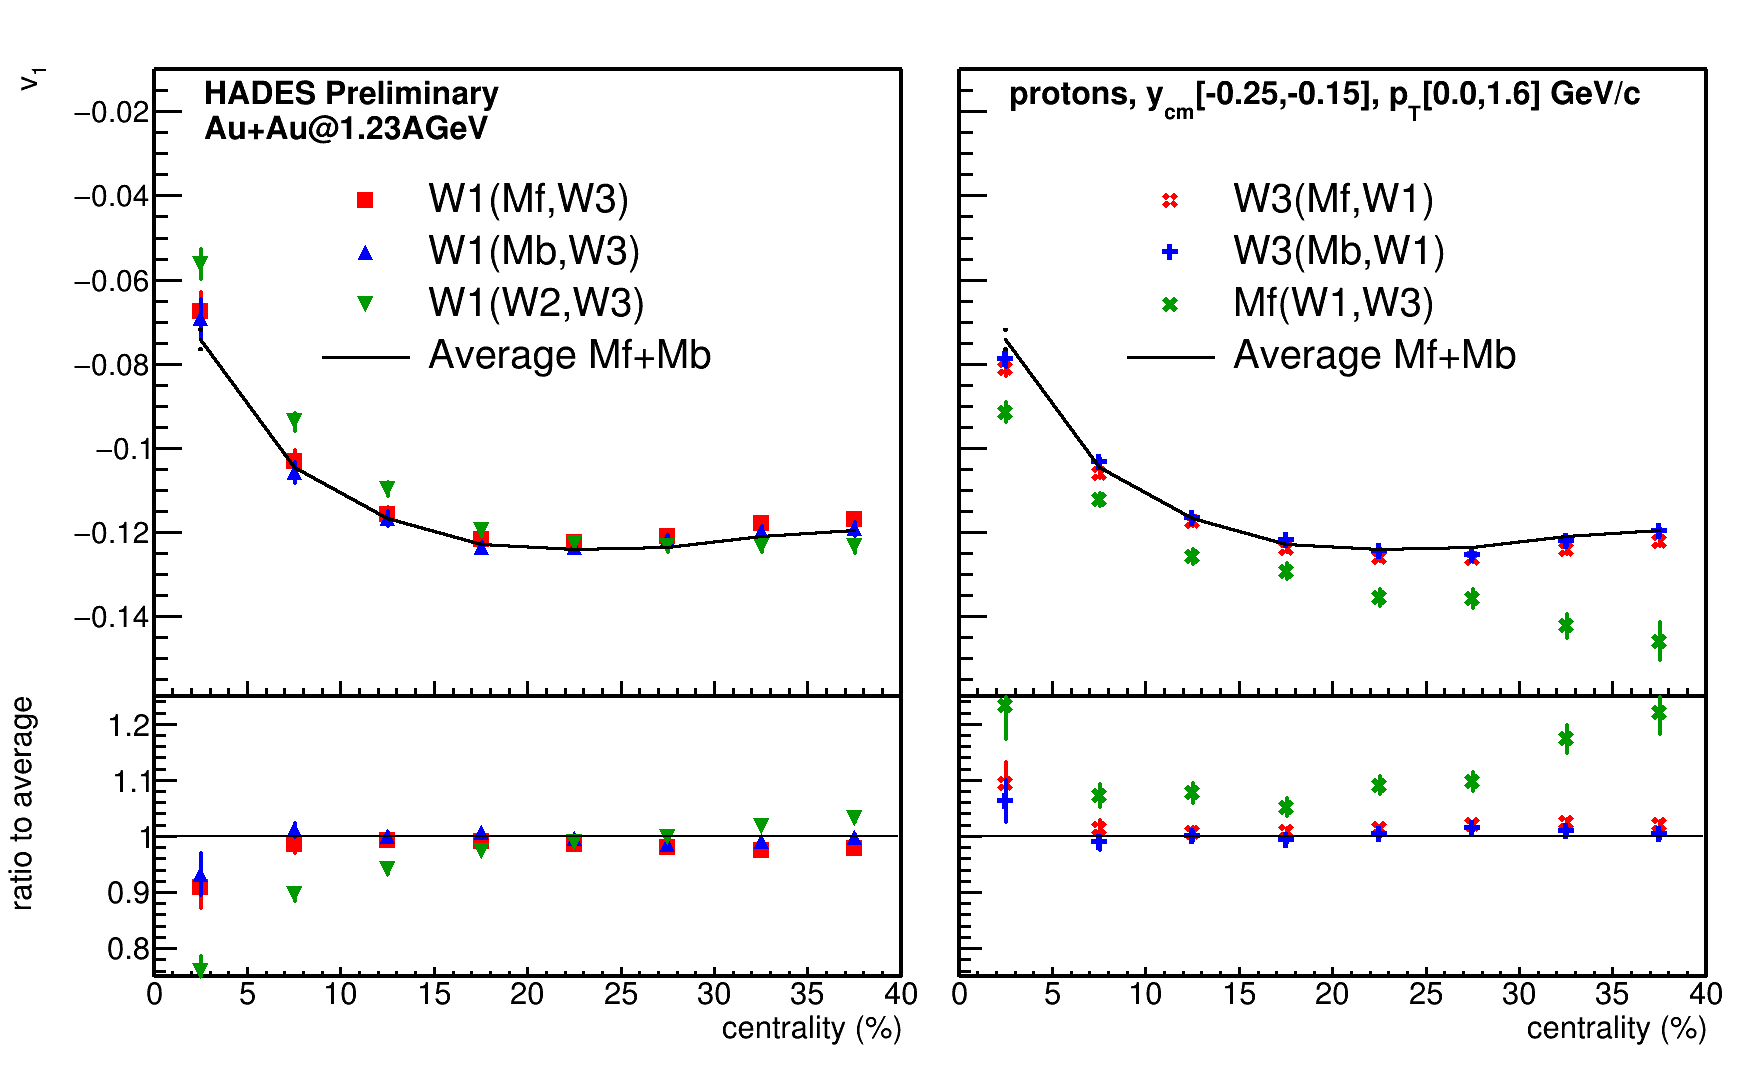
\includegraphics[width=0.75\linewidth]{images/W1AndW3Nucleus.png}
\caption{Направленный поток протонов $v_1$ рожденных в столкновении Au+Au при энергии $E_{kin}=$1.23$A$~ГэВ как функция центральности столкновения, измеренный при помощи различных комбинаций $Q_1$-векторов. Слева представлены значения $v_1$ протонов измеренный относительно внутреннего подсобытия W1, справа --- внешнего подсобытия W3 и подсобытия из треков заряженных частиц Mf. Черной линией представлено среднее результатов полученных при помощи разделенных по быстроте комбинаций.}
\label{fig:hades_w1w3}
\end{center}
\end{figure}

\subsection{Сравнение методов плоскости события и скалярного произведения}

Измерения направленного потока в~\cite{HADES:2020lob} были выполнены используя метод плоскости события. 
Для оценки возможной систематики, связанной с этим методом измерения $v_1$, направленный поток был рассчитан также методом скалярного произведеления.
Сравнение результатов полученных этими двумя методами позволит оценить вклад нелинейной зависимости $v_1\{EP\}$ от аксептанса установки и реального значения $v_1$.

На рисунке~\ref{fig:hades_ep_vs_sp} представлен направленный поток протонов рожденных в столкновениях Au+Au при энергии $E_{kin}=$1.23$A$~ГэВ как функция центральности, измеренный методом плоскости события и скалярного произведения. 
Значения $v_1$, полученные различными методами, хорошо согласуются между собой с учетом статистической ошибки. 
%
\begin{figure}[ht]
\begin{center}
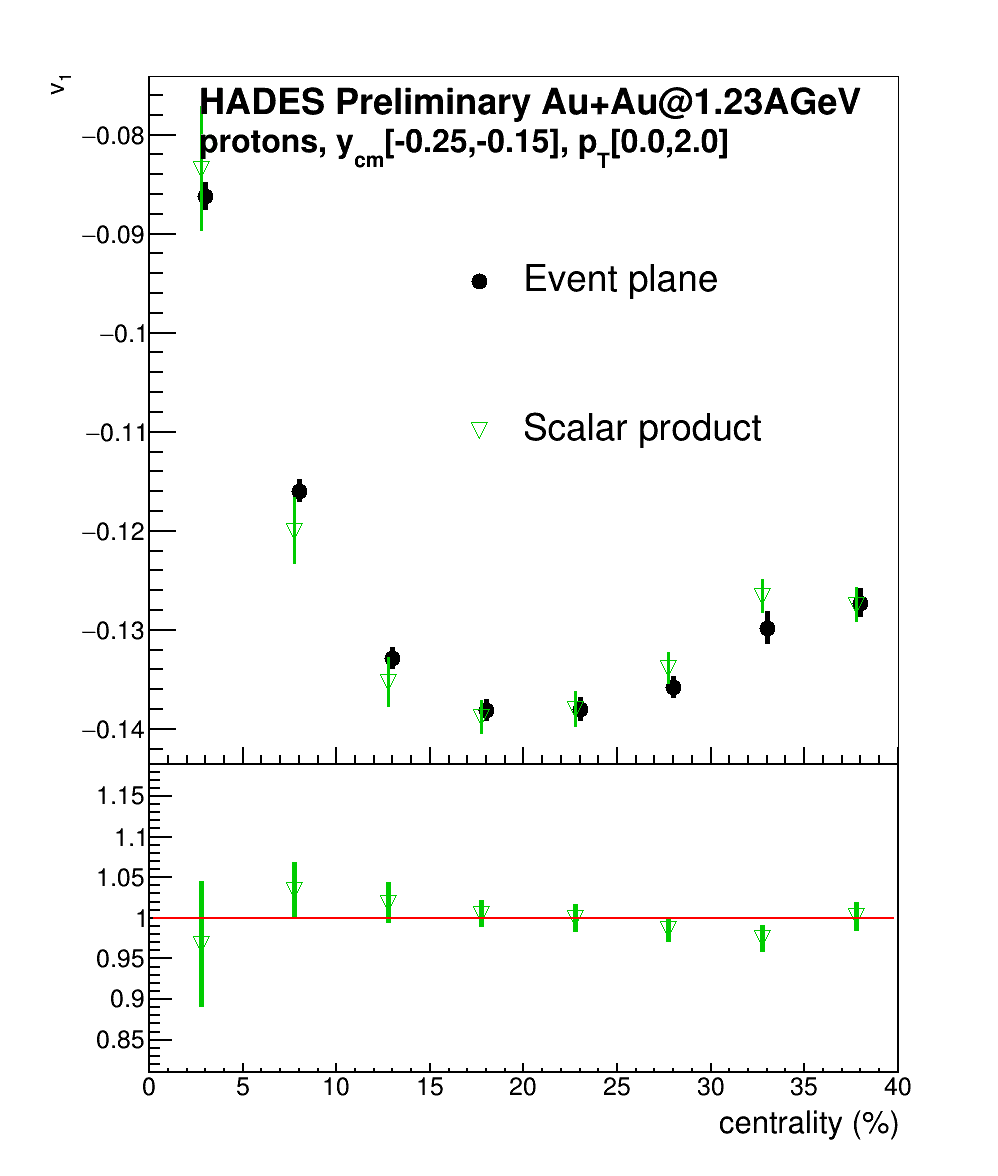
\includegraphics[width=0.45\linewidth]{images/EP_vs_SP.png}
\caption{Направленный поток протонов $v_1$, рожденных в столкновении Au+Au при энергии $E_{kin}=$1.23$A$~ГэВ как функция центральности столкновения. Результаты показаны для методов скалярного произведения (SP) и плоскости события (EP).}
\label{fig:hades_ep_vs_sp}
\end{center}
\end{figure}

\subsection{Сравнение методов случайных подсобытий и метода трёх подсобытий}

На рис.~\ref{fig:hades_rs_3s} показан направленный поток $v_1$ протонов, рожденных в столкновении Au+Au при энергии $E_{kin}=$1.23$A$~ГэВ (слева), Ag + Ag при энергии $E_{kin}=$1.23$A$~ГэВ (посередине) и Ag + Ag при энергии $E_{kin}=$1.58$A$~ГэВ (справа) как функция центральности столкновения. Результаты представлены для методов трех подсобытий и метода случайных подсобытий.
Для столкновений Au + Au при при энергии $E_{kin}=$1.23$A$~ГэВ (слева) разница между двумя методами вычисления корректировочного коэффициента разрешения составляет менее 5\% для среднецентральных столкновений.
Однако для меньшей системы столкновения, разница значительно больше. 
Это может быть объяснено меньшей множественностью рожденных частиц и спектаторов, и большем относительном вкладе непотоковых корреляций между $Q_1$-векторами, используемыми для расчета разрешения плоскости симметрии.
Наибольшая разница между двумя методами наблюдается для столкновений Ag + Ag при энергии $E_{kin}=$1.58$A$~ГэВ (справа).
Этот факт объясняется меньшим значением направленного потока $v_1$ спектаторов, отсюда больший относительный вклад непотоковых корреляций.
На основании этого наблюдения, можно сделать вывод о ненадёжности метода случайных подсобытий для более лёгких систем.
%
\begin{figure}[ht]
\begin{center}
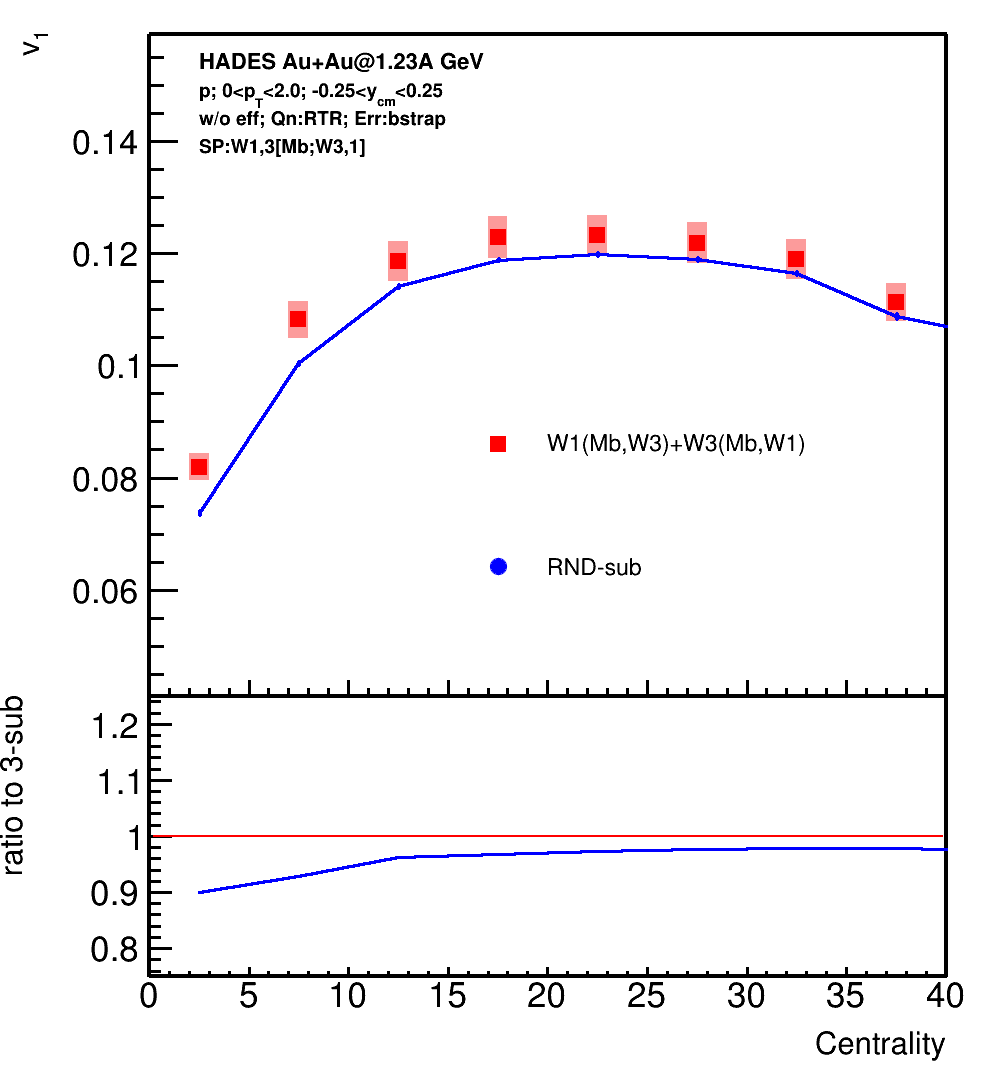
\includegraphics[width=0.3\linewidth]{images/v1_au123_3s_rnd.png}
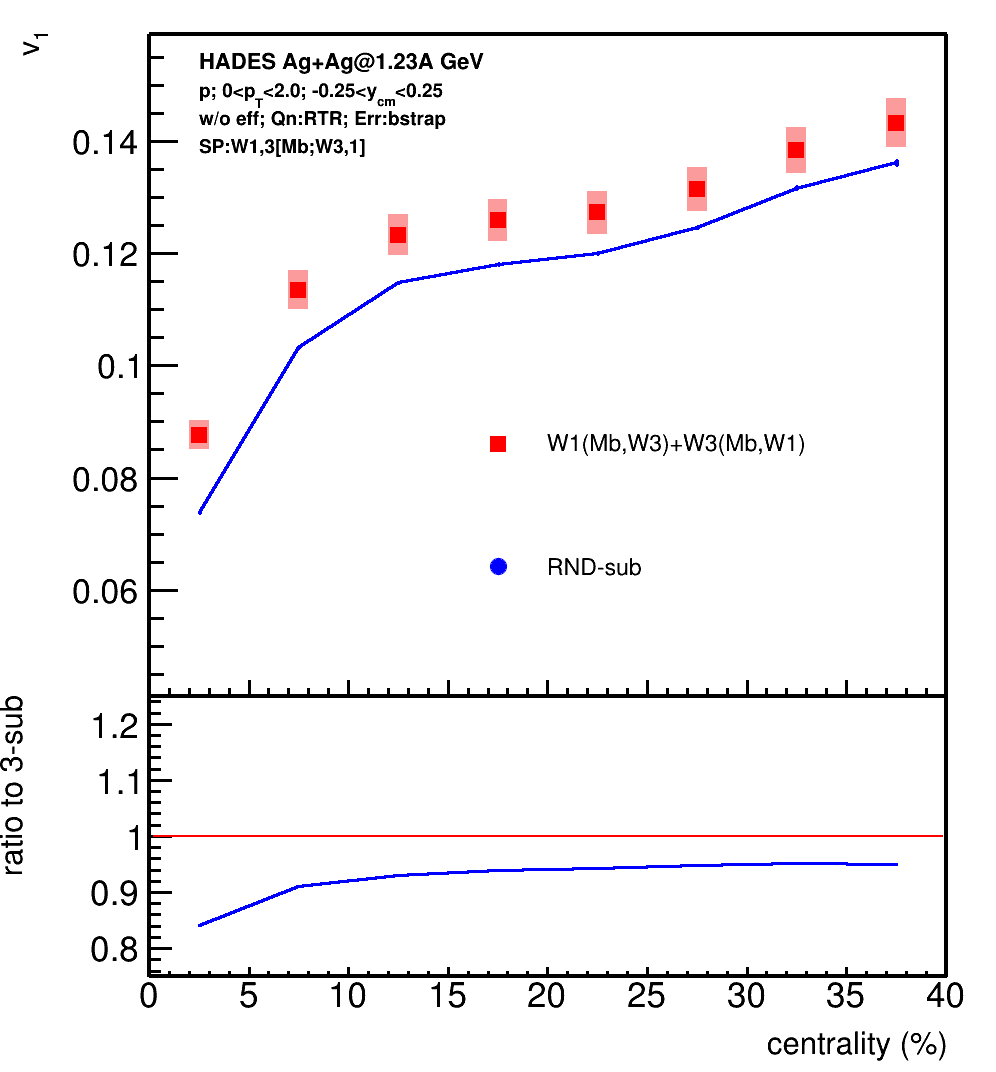
\includegraphics[width=0.3\linewidth]{images/v1_ag123_3s_rnd.png}
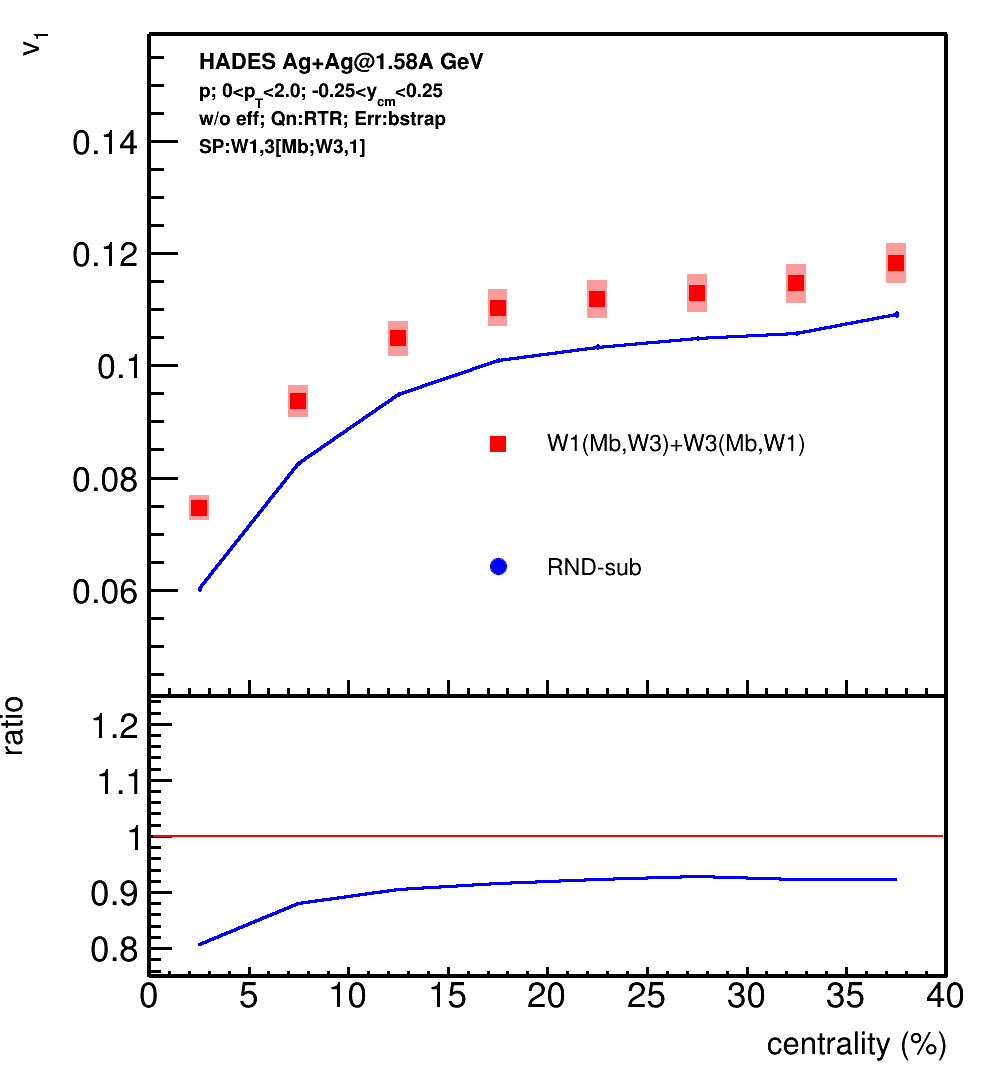
\includegraphics[width=0.3\linewidth]{images/v1_ag158_3s_rnd.png}
\caption{Направленный поток $v_1$ протонов, рожденных в столкновении Au+Au при энергии $E_{kin}=$1.23$A$~ГэВ (слева), Ag + Ag при энергии $E_{kin}=$1.23$A$~ГэВ (посередине) и Ag + Ag при энергии $E_{kin}=$1.58$A$~ГэВ (справа) как функция центральности столкновения. Результаты показаны для методов трех подсобытий и метода случайных подсобытий.}
\label{fig:hades_rs_3s}
\end{center}
\end{figure}

\subsection{Оценка итоговой систематики в значения $v_1$ от непотоковых корряляций}

На основании этих результатов, был сделан вывод о малом вкладе непотоковых корреляций в итоговые значения $v_n$ протонов и лёгких ядер, измеренных на установке HADES. 
Эти результаты легли в основу систематической ошибки измерений коллективной анизотропии и позволили опубликовать полученные данные~\cite{HADES:2020lob}.
На рис.~\ref{fig:hades_prl} приведен направленный поток $v_1$ протонов рожденных в столкновениях ядер золота при кинетической энергии пучка $E_{kin}=1.23A$~ГэВ как функция быстроты и поперечного импульса.
%
\begin{figure}[ht]
\begin{center}
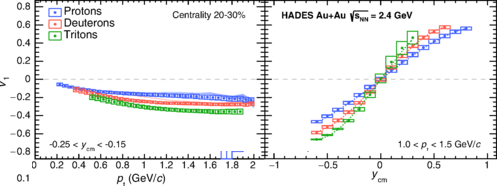
\includegraphics[width=0.75\linewidth]{images/HADES_prl.png}
\caption{Направленный поток ($v_1$) протонов, дейтронов и тритонов  рожденных в столкновении Au+Au при энергии $E_{kin}=$1.23$A$~ГэВ как функция быстроты (справа) и поперечного импульса (слева).}
\label{fig:hades_prl}
\end{center}
\end{figure}

\subsection{Сравнение результатов для $v_1$ протонов с опубликованными данными}

На рис.~\ref{fig:hades_v1_publ_comparison} представлено сравнение направленного потока измеренного для столкновений Au + Au при энергии $E_{kin}$=1.23$A$~ГэВ с опубликованными данными~\cite{HADES:2020lob}.
Направленный поток $v_1$ как функция быстроты (слева) и поперечного импульса (справа) хорошо согласуется с опубликованной зависимостью для протонов.
%
\begin{figure}[ht]
\begin{center}
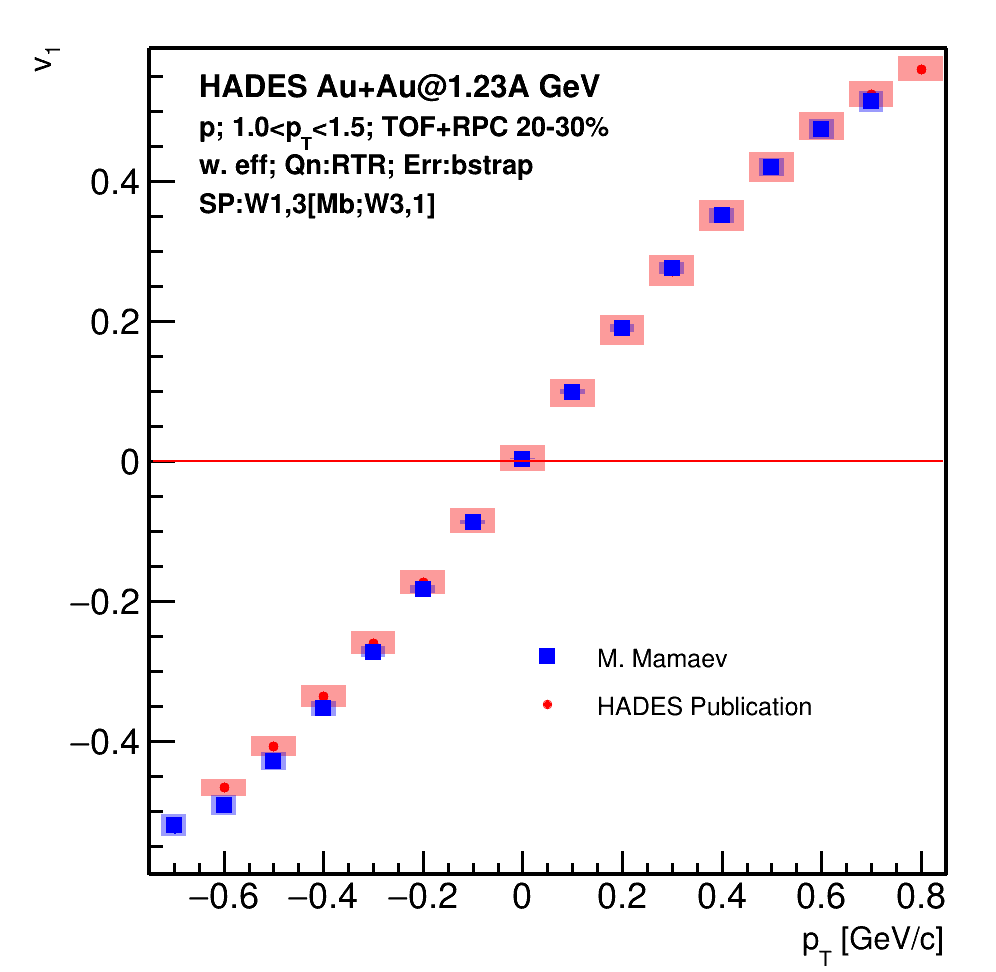
\includegraphics[width=0.45\linewidth]{images/v1_au123_publication_ycm.png}
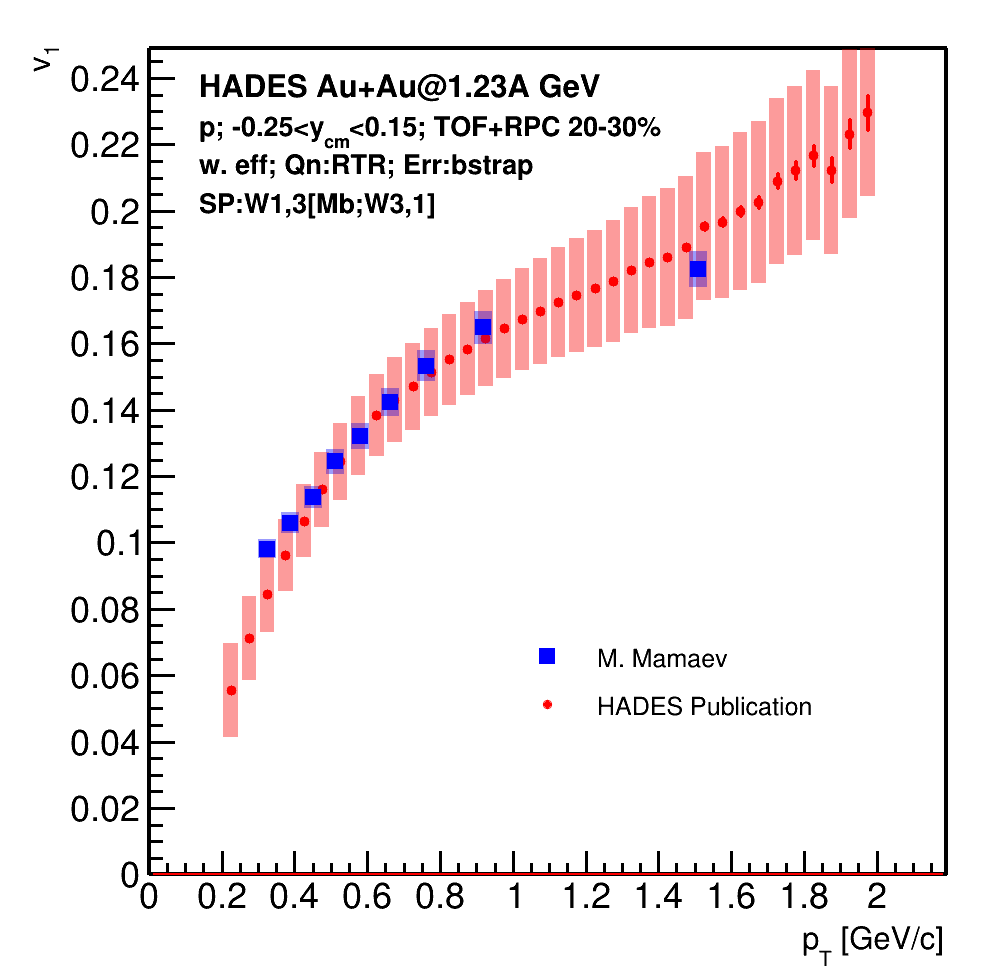
\includegraphics[width=0.45\linewidth]{images/v1_au123_publication_pT.png}
\caption{Направленный поток ($v_1$) протонов  рожденных в столкновении Au+Au при энергии $E_{kin}=$1.23$A$~ГэВ как функция быстроты (справа) и поперечного импульса (слева). Сравнение полученных результатов с опубликованными данными~\cite{HADES:2020lob}. }
\label{fig:hades_v1_publ_comparison}
\end{center}
\end{figure}

\subsection{Направленный поток $v_1$ протонов как функции быстроты и поперечного импульса в столкновениях Au + Au и Ag + Ag}

На рисунке~\ref{fig:hades_v1_ycm_pT} представлен направленный поток протонов $v_1$ как функция (слева) быстроты системы центра масс $y_{cm}$ и (справа) поперечного импульса $p_T$ для столкновений Au+Au при энергии $E_{kin}=$1.23$A$~ГэВ и Ag+Ag при энергиях $E_{kin}=$1.23$A$ и 1.58$A$~ГэВ.
Значения $v_1$ протонов, в столкновениях Au+Au и Ag+Ag при одной энергии, хорошо согласуются с учетом систематической ошибки. 
Протоны, рожденные в столкновениях Ag+Ag при большей энергии $E_{kin}=$1.58$A$~ГэВ обладают меньшим $v_1$, поскольку направленный поток чувствителен ко времени взаимодействия области перекрытия и остатков сталкивающихся ядер.
Чем меньше время взаимодействия (чем больше энергия столкновения) тем меньше итоговое значение направленного потока.

Модель JAM~\cite{nara2019jam} с импульсно зависимым потенциалом хорошо описывает магнитуду $v_1$ протонов и зависимость наблюдаемой от быстроты $y_{cm}$.
Однако модель не способна описать зависимость $v_1$ от поперечного импульса $p_T$.
%
\begin{figure}[ht]
\begin{center}
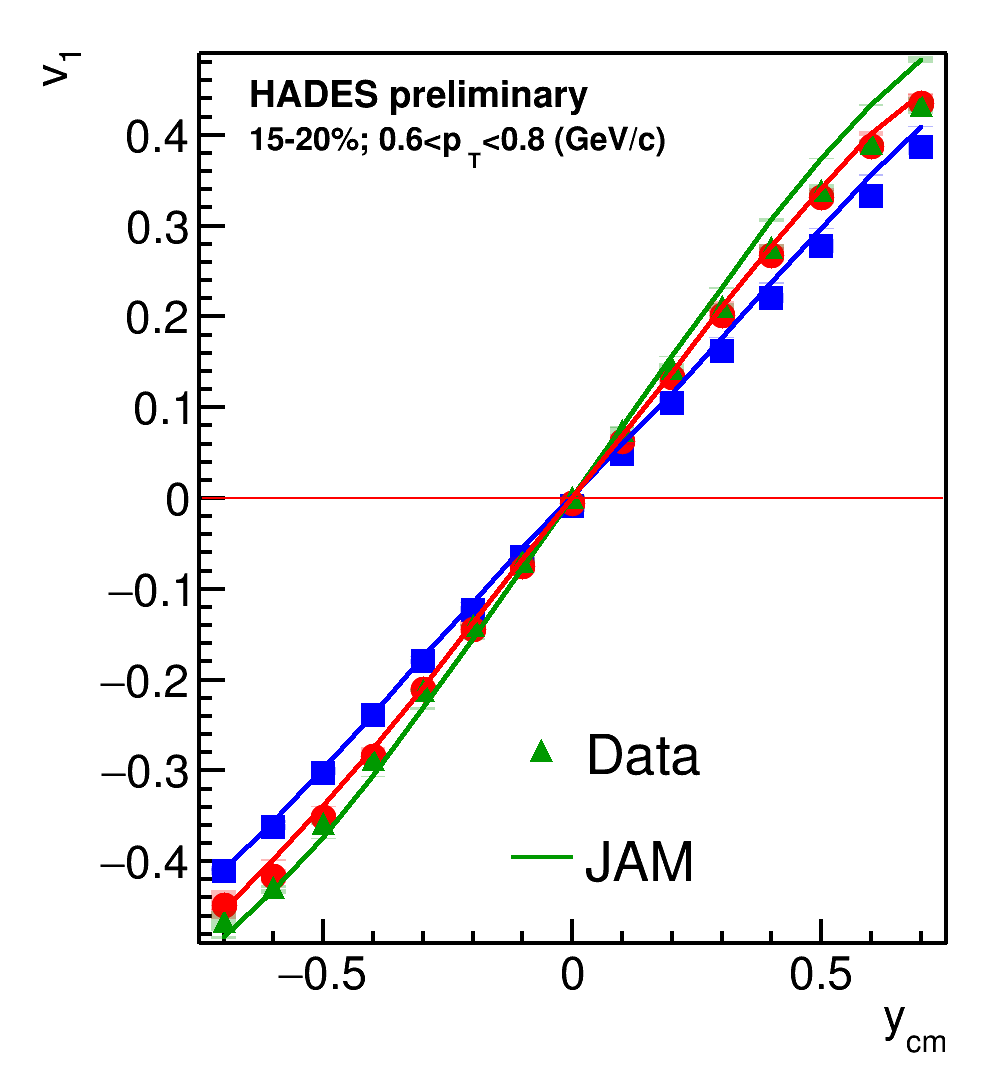
\includegraphics[width=0.45\linewidth]{images/v1_hades_ycm.png}
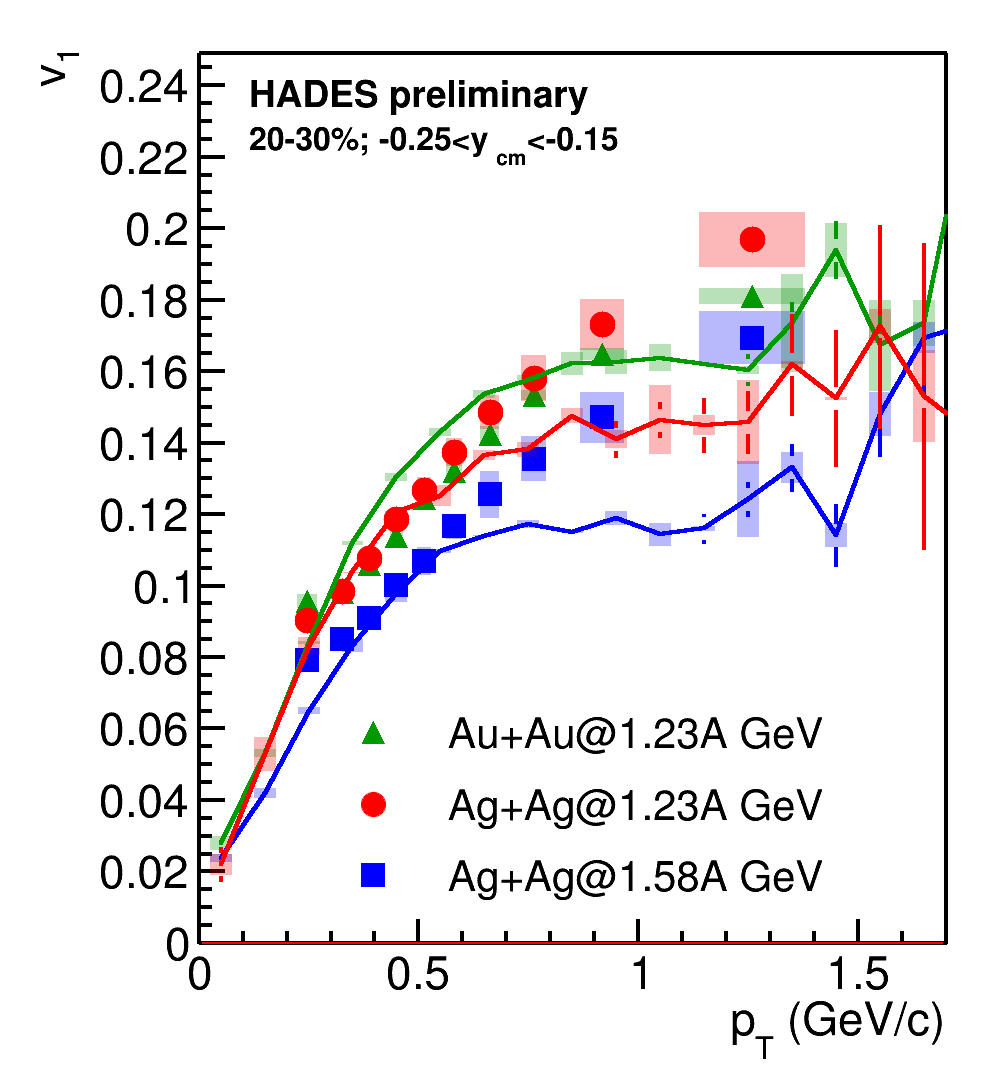
\includegraphics[width=0.45\linewidth]{images/v1_hades_pT.png}
\caption{Направленный поток протонов $v_1$ как фукция (слева) быстроты системы центра масс $y_{cm}$ и (справа) поперечного импульса $p_T$ для столкновений Au+Au при энергии $E_{kin}=$1.23$A$~ГэВ и Ag+Ag при энергиях $E_{kin}=$1.23$A$ и 1.58$A$~ГэВ. Линиями показаны данные, полученные из модели JAM с импульсно-зависимым потенциалом.}
\label{fig:hades_v1_ycm_pT}
\end{center}
\end{figure}

\subsection{Проверка теоретических предсказаний эффектов масштабирования $v_1$ протнов в реалистичной модели Jet A-A Model (JAM)}

На рис.~\ref{fig:hades_model_ycm_scaling} представлены теоретические предсказания значений направленного потока протонов $v_1$ как функция быстроты столкновения $y_{cm}$ (слева) и быстроты, нормированной на быстроту пучка $y'=y_{cm}/y_{beam}$ (справа) из модели JAM.
Результаты для различных систем при одной энергии столкновения хорошо согласуются между собой и с экспериментальными данными для $v_1$ в столкновениях Au + Au при энергии $E_{kin}$=1.23$A$~ГэВ.
После нормировки быстроты столкновения на быстроту пучка, результаты можно описать единой кривой.
Этот факт свидетельствует о едином механизме образования направленного потока в данной области энергии в тяжелых системах.
%
\begin{figure}[ht]
\begin{center}
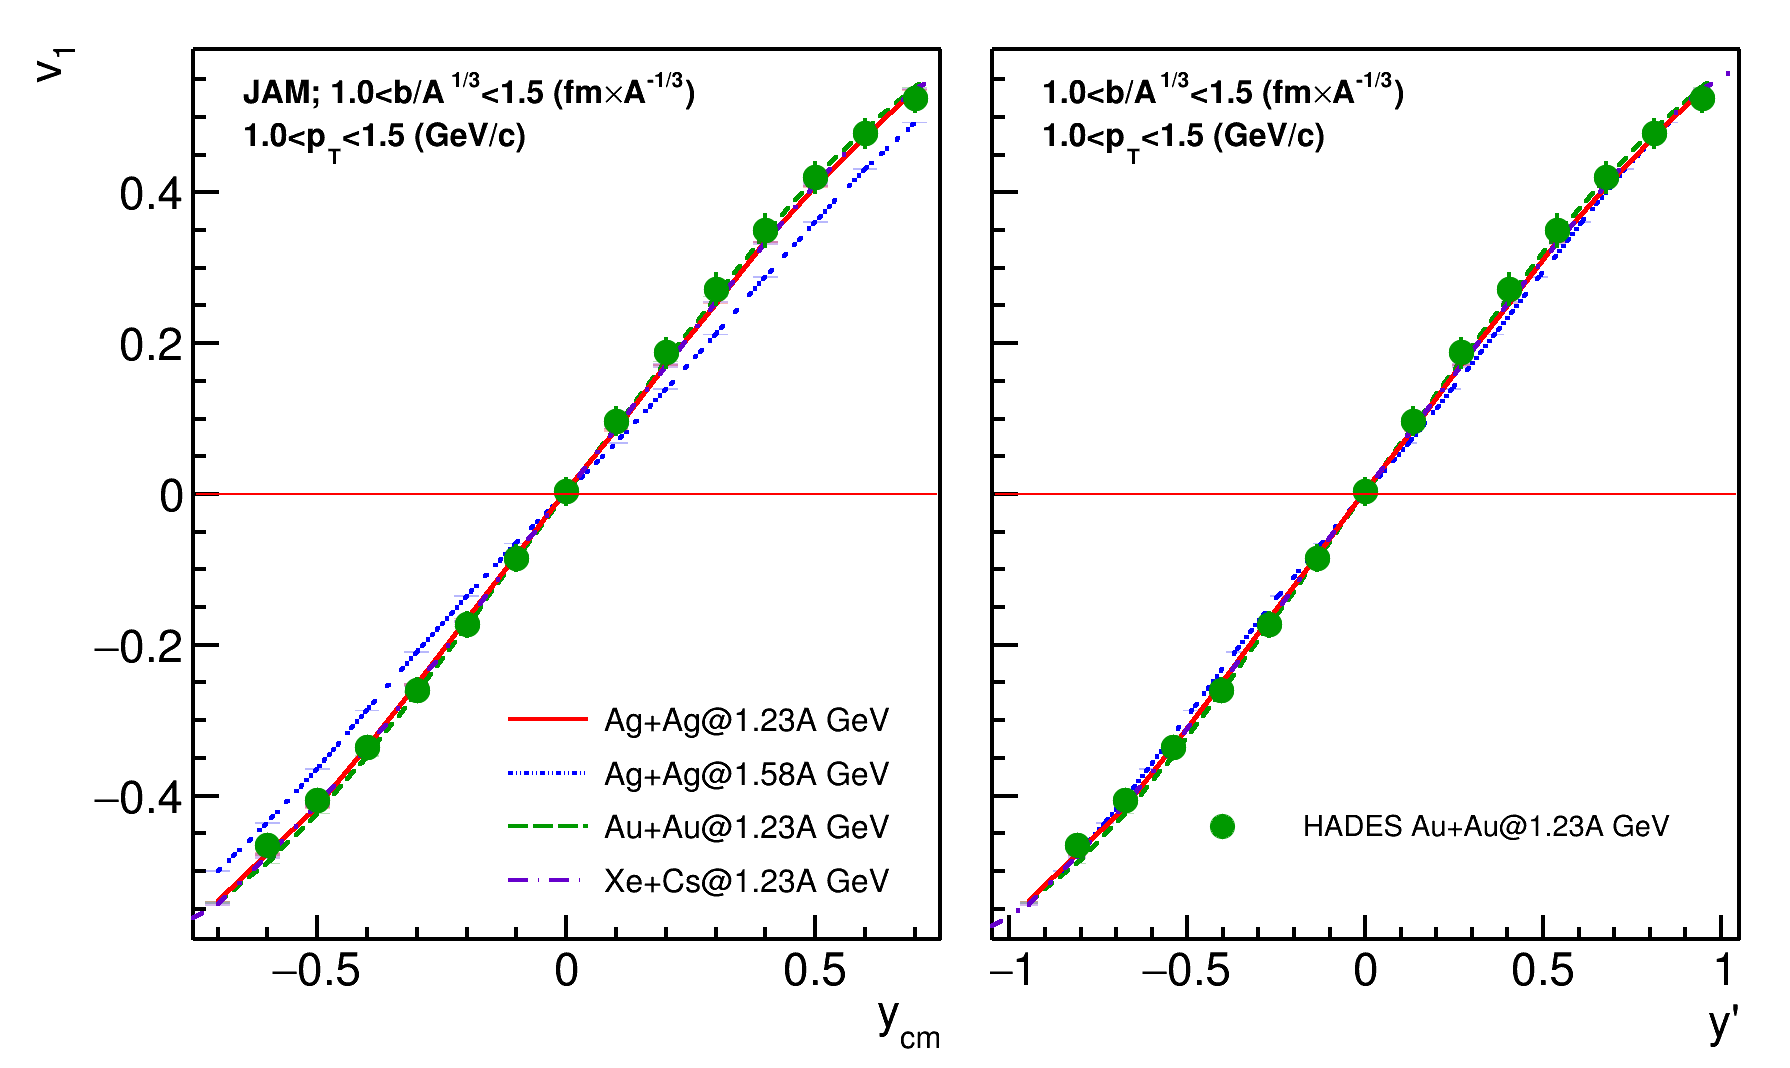
\includegraphics[width=0.95\linewidth]{images/v1_hades_model_ycm_scaling.png}
\caption{Направленный поток протонов $v_1$ как функция быстроты столкновения $y_{cm}$ (слева) и быстроты, нормированной на быстроту пучка $y'=y_{cm}/y_{beam}$ (справа) из модели JAM.}
\label{fig:hades_model_ycm_scaling}
\end{center}
\end{figure}

\subsection{Проверка эффектов масштабирования наклона направленного потока протонов в средних быстротах $dv_1/dy|_{y=0}$}

Зависимость направленного потока протонов $v_1$ как функция быстроты была параметризована кубической функцией $v_1(y_{cm}) = a_0 + a_1 y_{cm} + a_3 y_{cm}^3$. 
Затем наклон направленного потока протонов в нуле быстроты $dv_1/dy_{cm}|_{y_{cm}=0}$ был извлечен как параметр $a_1$.
На рис.~\ref{fig:hades_dv1dy_many_plot} слева приведена зависимость наклона направленного потока в нуле быстроты как функция центральности столкновения.
Наклоны $dv_1/dy_{cm}|_{y_{cm}=0}$ протонов для столкновений Au+Au и Ag+Ag при одной энергии хорошо согласуются между собой за исключением наиболее центральных событий. 
Поскольку при большей энергии время пролета двух ионов меньше, наклон направленного потока протонов в столкновениях Ag+Ag при энергии $E_{kin}=$1.58$A$~ГэВ заметно меньше.
Для коррекции на время пролета, наклон направленного потока протонов $dv_1/dy_{cm}|_{y_{cm}=0}$ был нормирован на быстроту пучка $dv_1/dy_{cm}|_{y_{cm}=0} \times y_{b} = dv_1/dy'|_{y'=0}$, где $y_{b}$ --- быстрота пучка (0.74 для $E_{kin}=$1.23$A$~ГэВ и 0.82 для  $E_{kin}=$1.58$A$~ГэВ) и $y'=y_{cm}/y_b$.
Наклон направленного потока протонов нормированный на быстроту $dv_1/dy'|_{y'=0}$ пучка как функция центральности показан на рис.~\ref{fig:hades_dv1dy_many_plot} в центре. 
За исключением наиболее центральных событий, зависимость наклона от центральности описывается одной кривой для всех трех наборов данных.
В каждом классе центральности был вычислен средний прицельный параметр $\langle b \rangle$. 
Радиус ядра пропорционален корню кубическому из массового числа $r_N \propto A^{1/3}$.
Для устранения зависимости от размера сталкиваемых ядер, средний прицельный параметр в классе центральности был нормирован на $A^{1/3}$.
Наклон направленного потока протонов, нормированный на быстроту пучка $dv_1/dy'|_{y'=0}$ как функция относительного прицельного параметра  $ \langle b \rangle / A^{1/3}$ представлен на рис~\ref{fig:hades_dv1dy_many_plot} справа.
Данное преобразование улучшило согласие зависимостей наклона в центральных событиях. 
%
\begin{figure}[ht]
\begin{center}
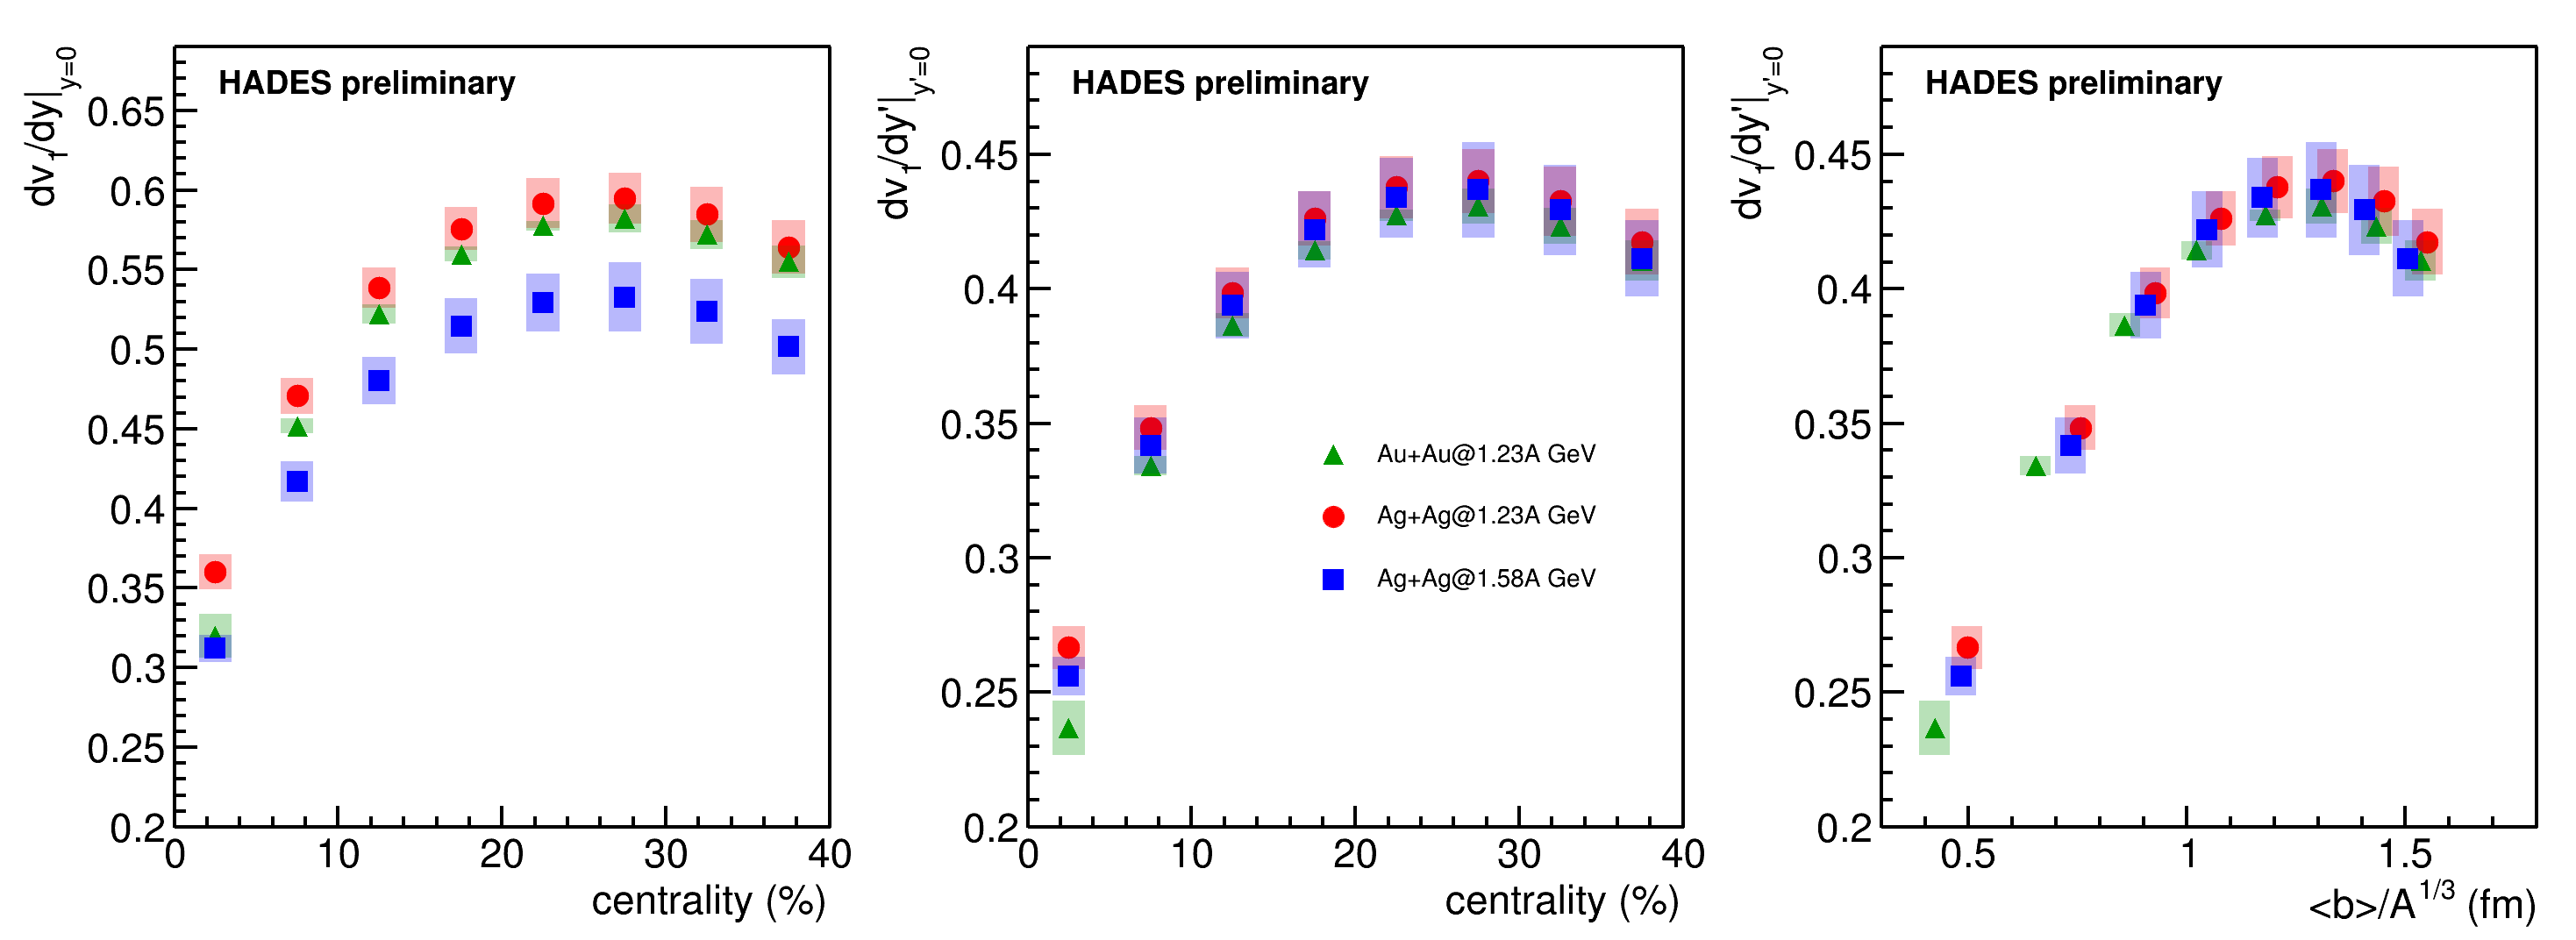
\includegraphics[width=0.9\linewidth]{images/dv1dy_many_plot.png}
\caption{ 
(Слева) Наклон направленного потока в нуле быстроты $dv_1/dy|_{y_{cm}=0}$ как функция центральности столкновений;
(посередине) наклон направленного потока в нуле быстроты нормированный на быстроту пучка $dv_1/dy|_{y'=0}$ как функция центральности столкновений;
(справа) наклон направленного потока в нуле быстроты нормированный на быстроту пучка $dv_1/dy|_{y'=0}$ как функция среднего прицельного параметра в классах центральности
для столкновений Au+Au при энергии $E_{kin}=$1.23$A$~ГэВ и Ag+Ag при энергиях $E_{kin}=$1.23$A$ и 1.58$A$~ГэВ. }
\label{fig:hades_dv1dy_many_plot}
\end{center}
\end{figure}

\subsection{Эффекты масштабирования для направленного потока $v_1$ протонов как функция поперечного импульса}

На рис.~\ref{fig:v1_pT_scaling} представлена зависимость от поперечного импульса $p_T$ направленного потока $v_1$ (слева) и направленного потока, нормированного на наклон в средних быстротах $v_1/dv_1/dy|_{y=0}$ (справа).
Результаты до нормировки для столкновений Au + Au и Ag + Ag при одной энергии находятся в хорошем согласии с учетом систематической ошибки.
Результаты для столкновений Ag + Ag при большей энергии систематически ниже, поскольку величина направленного потока $v_1$ зависит от времени пролета сталкивающихся ядер $t_{pass}$, которая меньше при более высокой энергии.
После нормировки (см. справа), все результаты ложатся на единую кривую.
Этот факт может свидетельствовать о едином механизме образования направленного потока в этой области энергии.
\begin{figure}[ht]
\begin{center}
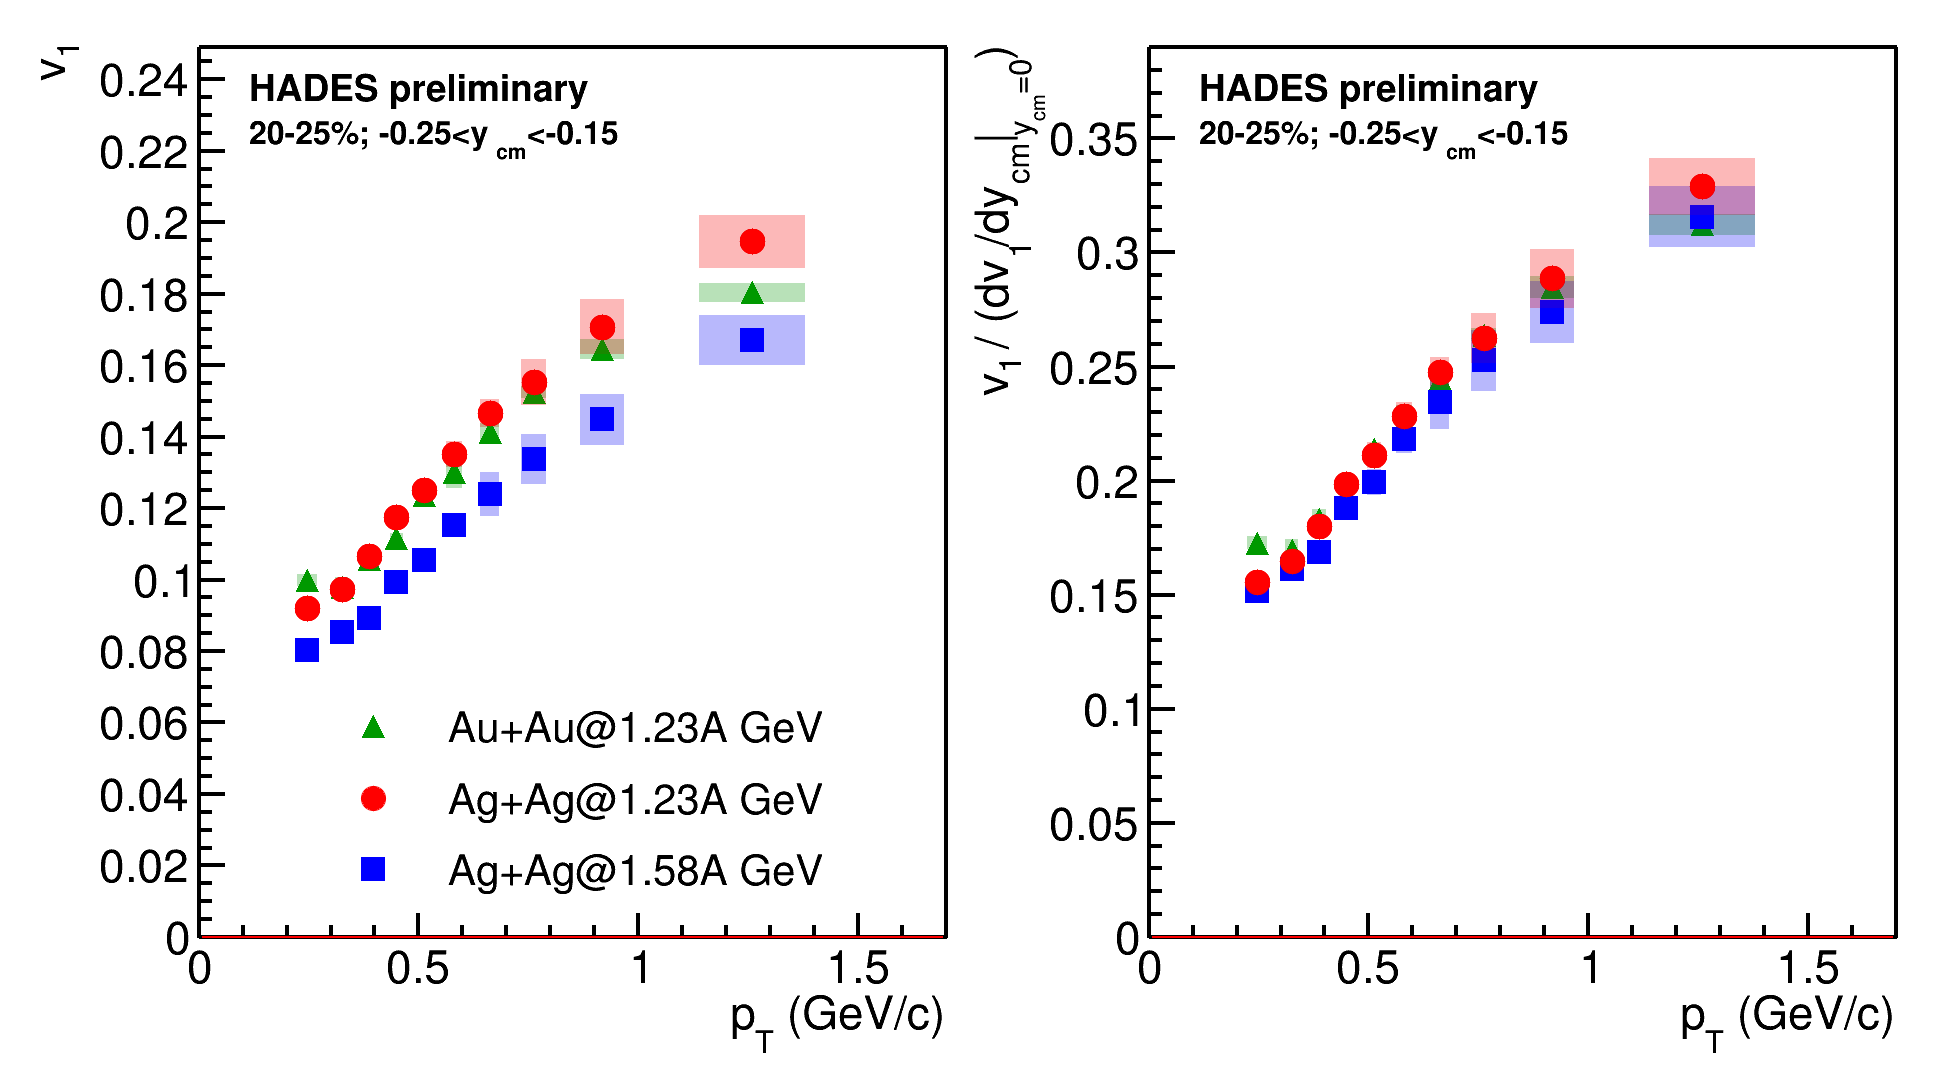
\includegraphics[width=0.9\linewidth]{images/v1_hades_pT_scaling.png}
\caption{ 
    Направленный поток протонов $v_1$ как функция поперечного импульса $p_T$. Слева: направленный поток $v_1$, справа: направленный поток, нормированный на наклон в средних быстротах $v_1/dv_1/dy|_{y=0}$.
}.
\label{fig:v1_pT_scaling}
\end{center}
\end{figure}

Описанный выше эффект был также обнаружен в модели с импульсно-зависимым потенциалом JAM.
На рис.~\ref{fig:v1_model_pT_scaling} представлена зависимость от поперечного импульса $p_T$ направленного потока $v_1$ (слева) и направленного потока, нормированного на наклон в средних быстротах $v_1/dv_1/dy|_{y=0}$ (справа) для различных систем из модели JAM.
До нормировки результаты для направленного потока как функция $p_T$ для столкновений при одной энергии так же находятся в довольно хорошем согласии.
После нормировки, теоретические предсказания так же ложатся на единую кривую. 
\begin{figure}[ht]
\begin{center}
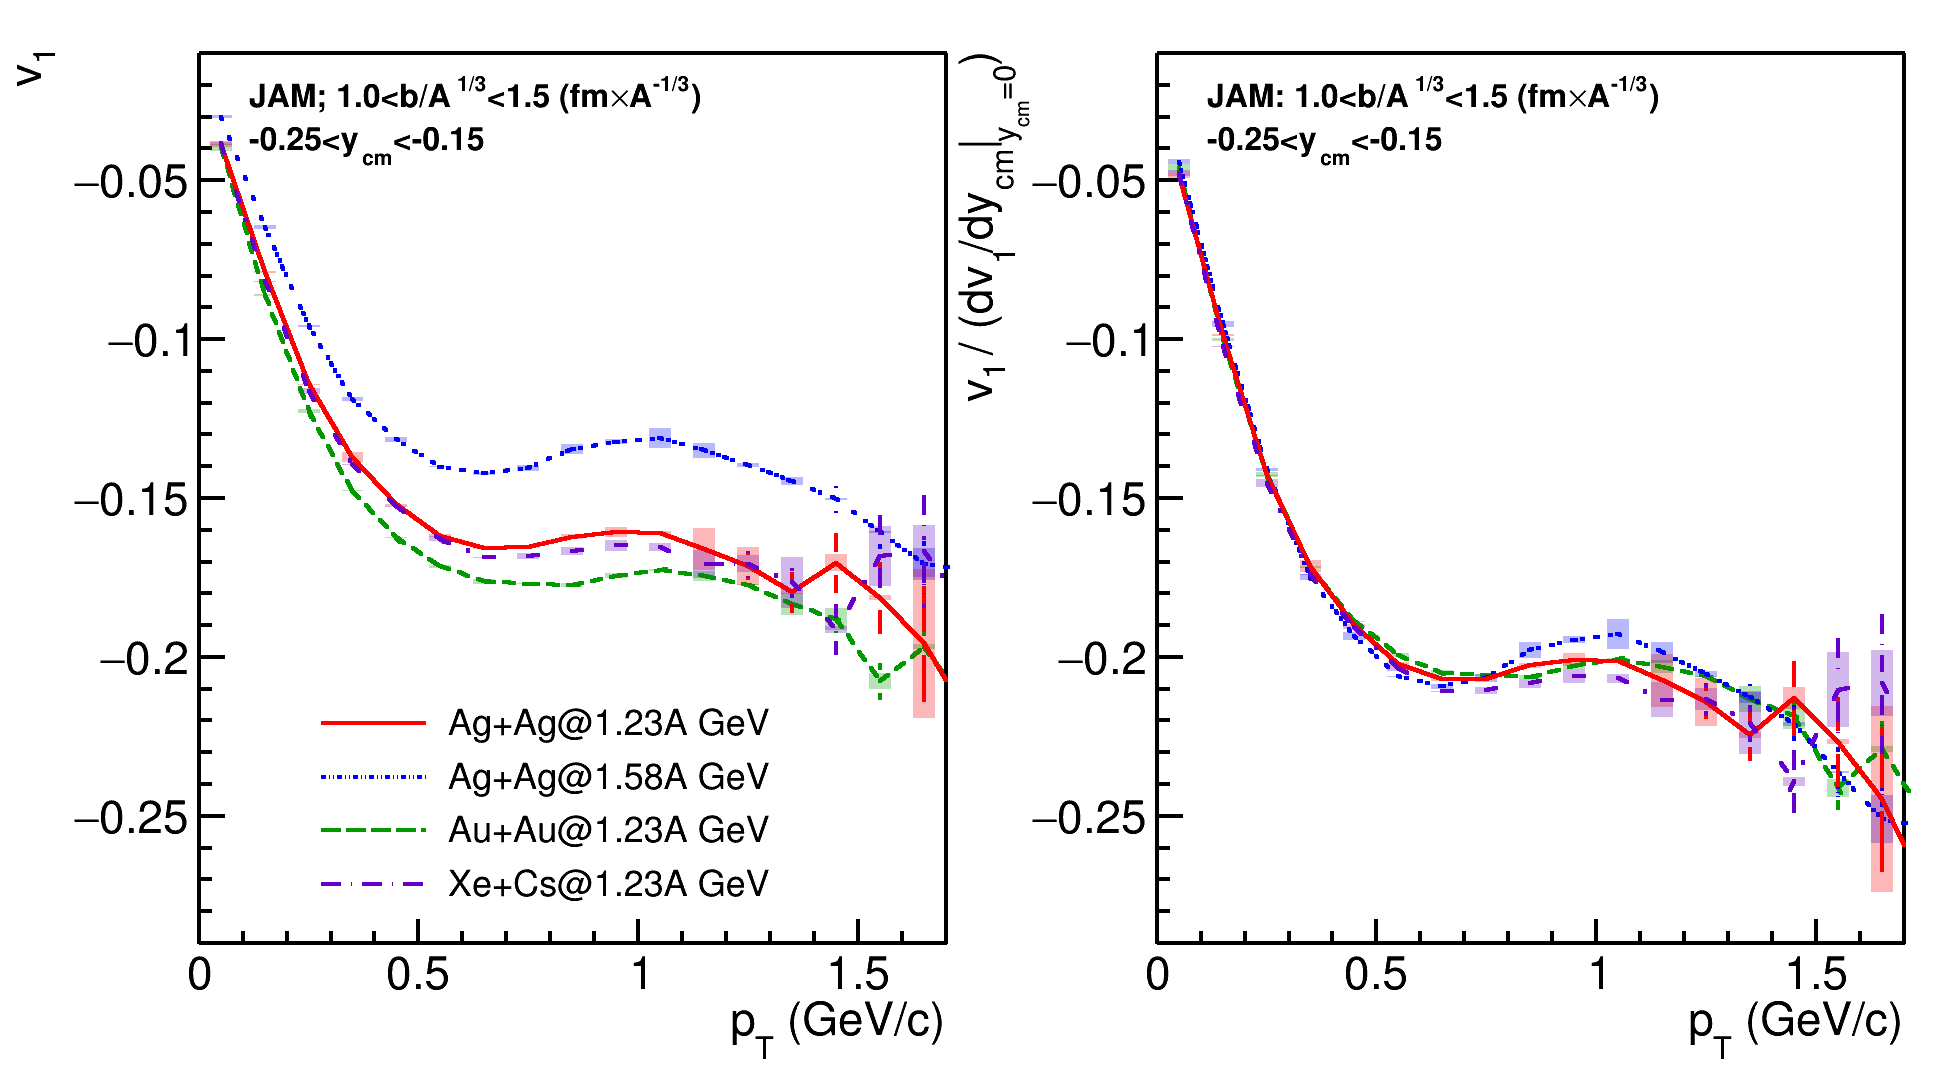
\includegraphics[width=0.9\linewidth]{images/v1_hades_model_pT_scaling.png}
\caption{ 
    Направленный поток протонов $v_1$ как функция поперечного импульса $p_T$ в модели JAM для различных сталкиваемых систем. Слева: направленный поток $v_1$, справа: направленный поток, нормированный на наклон в средних быстротах $v_1/dv_1/dy|_{y=0}$.
}.
\label{fig:v1_model_pT_scaling}
\end{center}
\end{figure}

\subsection{Сравнение измеренного наклона направленного потока протонов в средних быстротах с мировыми данными}

Сравнение полученных значений наклона направленного потока протонов $dv_1/dy|_{y_{cm}=0}$ с существующими результатами показано на рис.~\ref{fig:hades_dv1_dy_sqrt_snn}.
Значения $dv_1/dy|_{y_{cm}=0}$ протонов в столкновениях \au{} при $E_{kin}=$1.23$A$~ГэВ и \ag{} при $E_{kin}=$1.23$A$ и  при $E_{kin}=$1.58$A$~ГэВ согласуются с измерениями с ранее доступными данными с других экспериментов.
%
\begin{figure}[ht]
\begin{center}
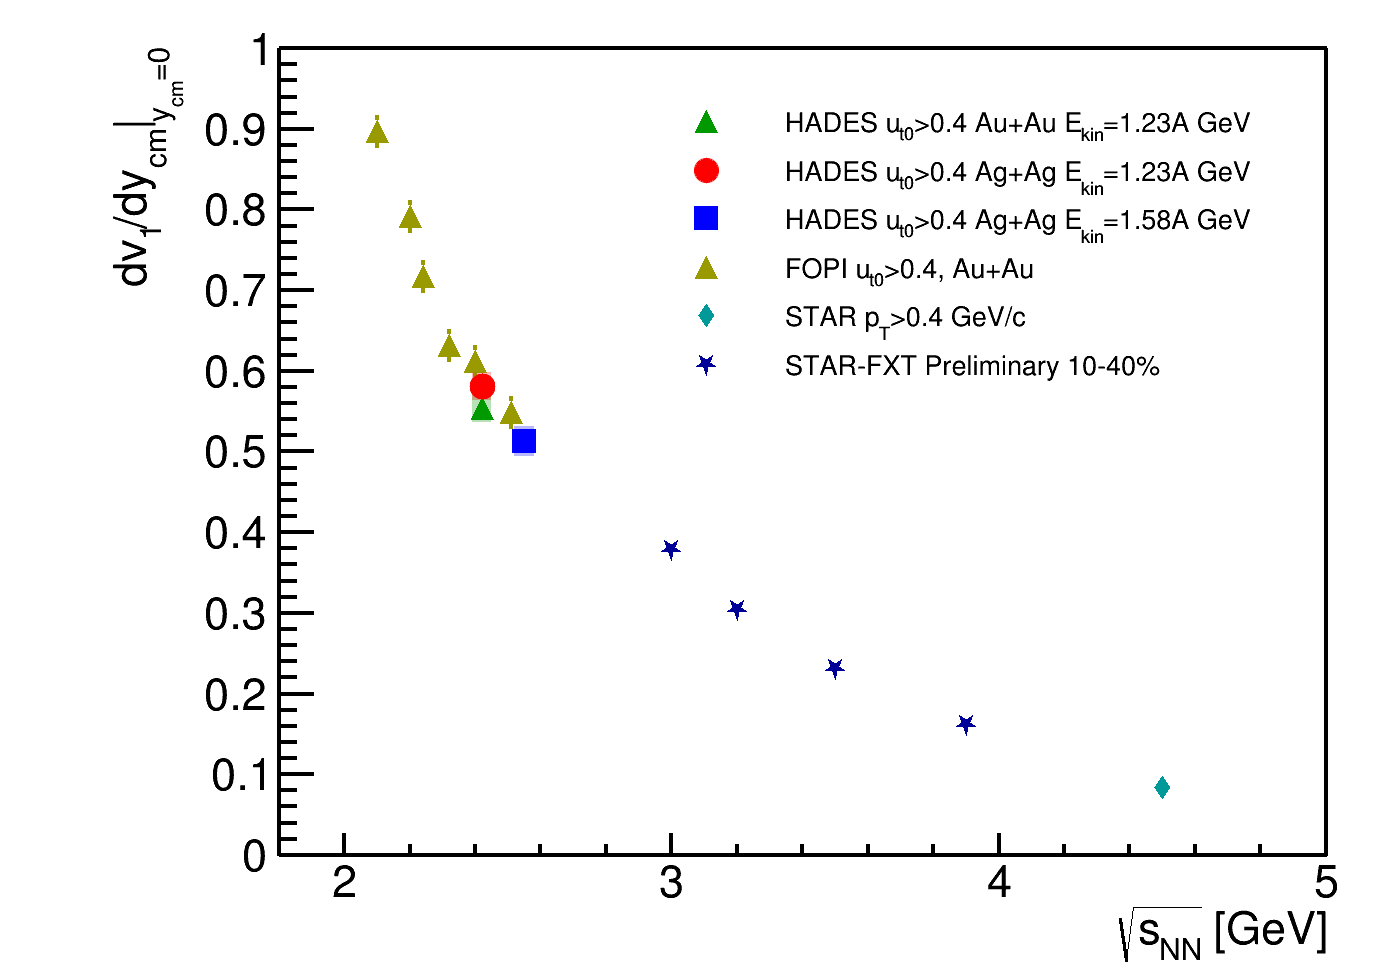
\includegraphics[width=0.9\linewidth]{images/dv1_dy_sqrt_snn.png}
\caption{ 
    Направленный поток протонов $dv_1/dy|_{y_{cm}=0}$ как функция энергии столкновения $\sqrt{s_{NN}}$. Экспериментальные значения наклона направленного потоа были взяты из следующих публикаций: E895~\cite{E895:2000maf}, FOPI~\cite{FOPI:2011aa}, STAR~\cite{STAR:2020dav}.
}
\label{fig:hades_dv1_dy_sqrt_snn}
\end{center}
\end{figure}

\section{Результаты анализа Монте-Карло моделирования эксперимента BM@N}

\subsection{Коррекция на азимутальную неоднородность аксептанса установки}

Эффект применения коррекций на азимутальную неоднородность детектора представлен на рис~\ref{fig:bmn_components}.
%
\begin{figure}[ht]
\begin{center}
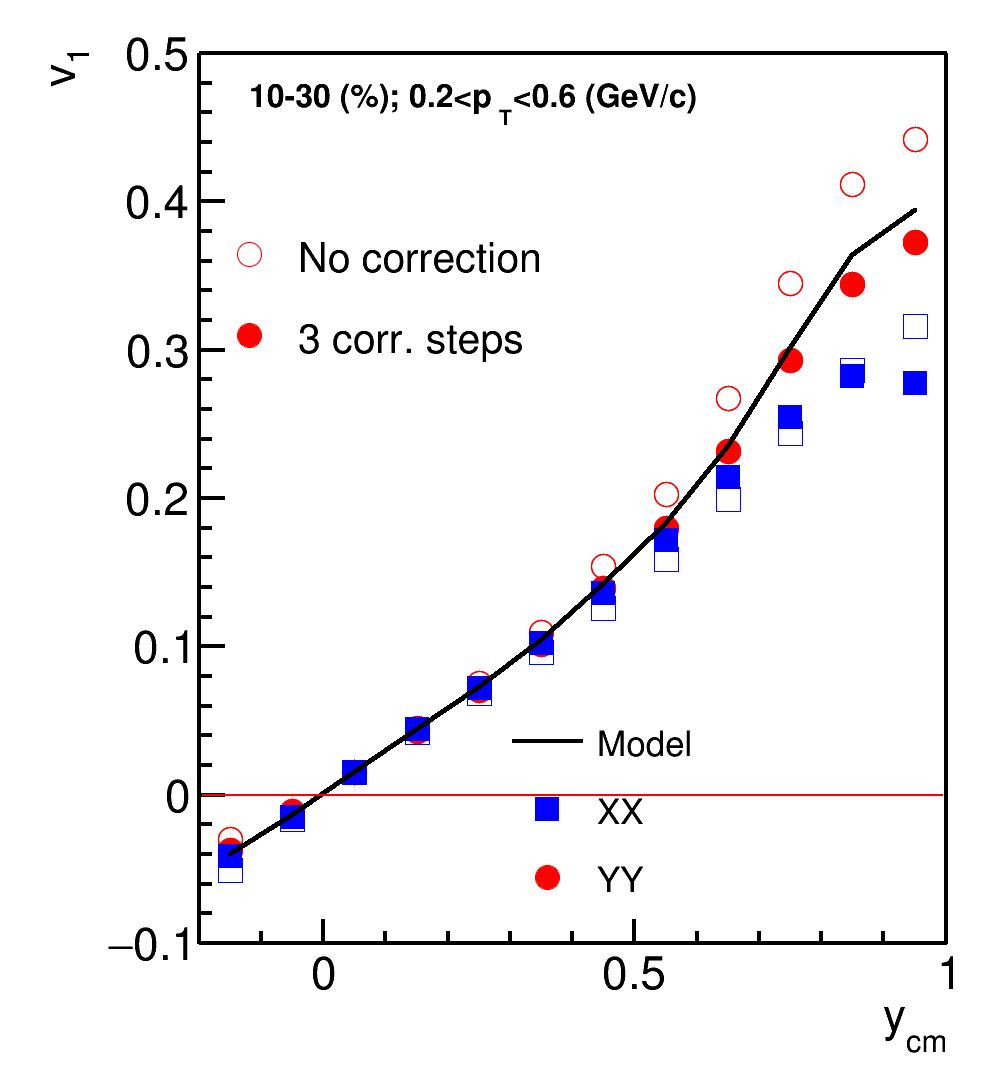
\includegraphics[width=0.45\linewidth]{images/v1_proton_correction_rapidity.png}
\caption{Сравнение направленного потока $v_1$ протонов рожденных в Монте-Карло моделировании столкновений Xe+Cs в эксперименте BM@N. Направленный поток получен с использованием различных компонент $u_1$-вектора. Разными маркерами обозначены результаты до и после коррекции на азимутальную неоднородность аксептанса детектора. }
\label{fig:bmn_components}
\end{center}
\end{figure}

Результаты получены для реалистичного моделирования отклика детектора с использованием программного пакета GEANT4.
Разными цветами обозначен результат $v_1$ протонов, полученный с использованием различных компонент $u_1$-вектора. 
Маркеры обозначают результаты до и после коррекции на азимутальную неоднородность детектора.
Черной линией обозначена зависимость $v_1$ протонов извлеченная напрямую из модели без реконструкции.
После применения 3 ступеней коррекции, результаты полученные при помощи $YY$ корреляции $u_1$ и $Q_1$-векторов, хорошо согласуются с результатами извлеченными напрямую из модели.
Напротив, $v_1$, посчитанный с использованием $XX$-компонент, расходится с модельной зависимостью $v_1$ от быстроты. 
Причиной может служить отклонение частиц в направлении оси $x$ в магнитном поле. 
В связи с этим, в дальнейшем для анализа будет использованы лишь корреляции $YY$-компонент $u_1$ и $Q_1$-векторов.

\subsection{Вычисление разрешения плоскости симметрии}

На рис.~\ref{fig:bmn_combinations} представлено разрешение плоскости симметрий $F1$, $F2$, $F3$ (слева направо). 
Аналогично, разрешение посчитанное с использованием комбинаций, не разделенных по быстроте $Q_1$-векторов (к примеру, $F1(F2,F3)$), отличается от значений рассчитанных при помощи комбинаций со значительным разделением по быстроте (к примеру, $F1(Tp,F3)$).
Значения $R_1$, полученные при помощи разделенных по быстроте комбинаций, согласуются между собой в пределах статистической ошибки для всех трех плоскостей симметрии. 
Значительное отличие разрешений, полученных с использованием комбинаций не разделенных по быстроте $Q_1$-векторов, может быть объяснено распространением адронного ливня в поперечном направлении, что вызывает дополнительные корреляции между векторами $F1$ и $F2$, и $F1$ и $F3$.
%
\begin{figure}[ht]
\begin{center}
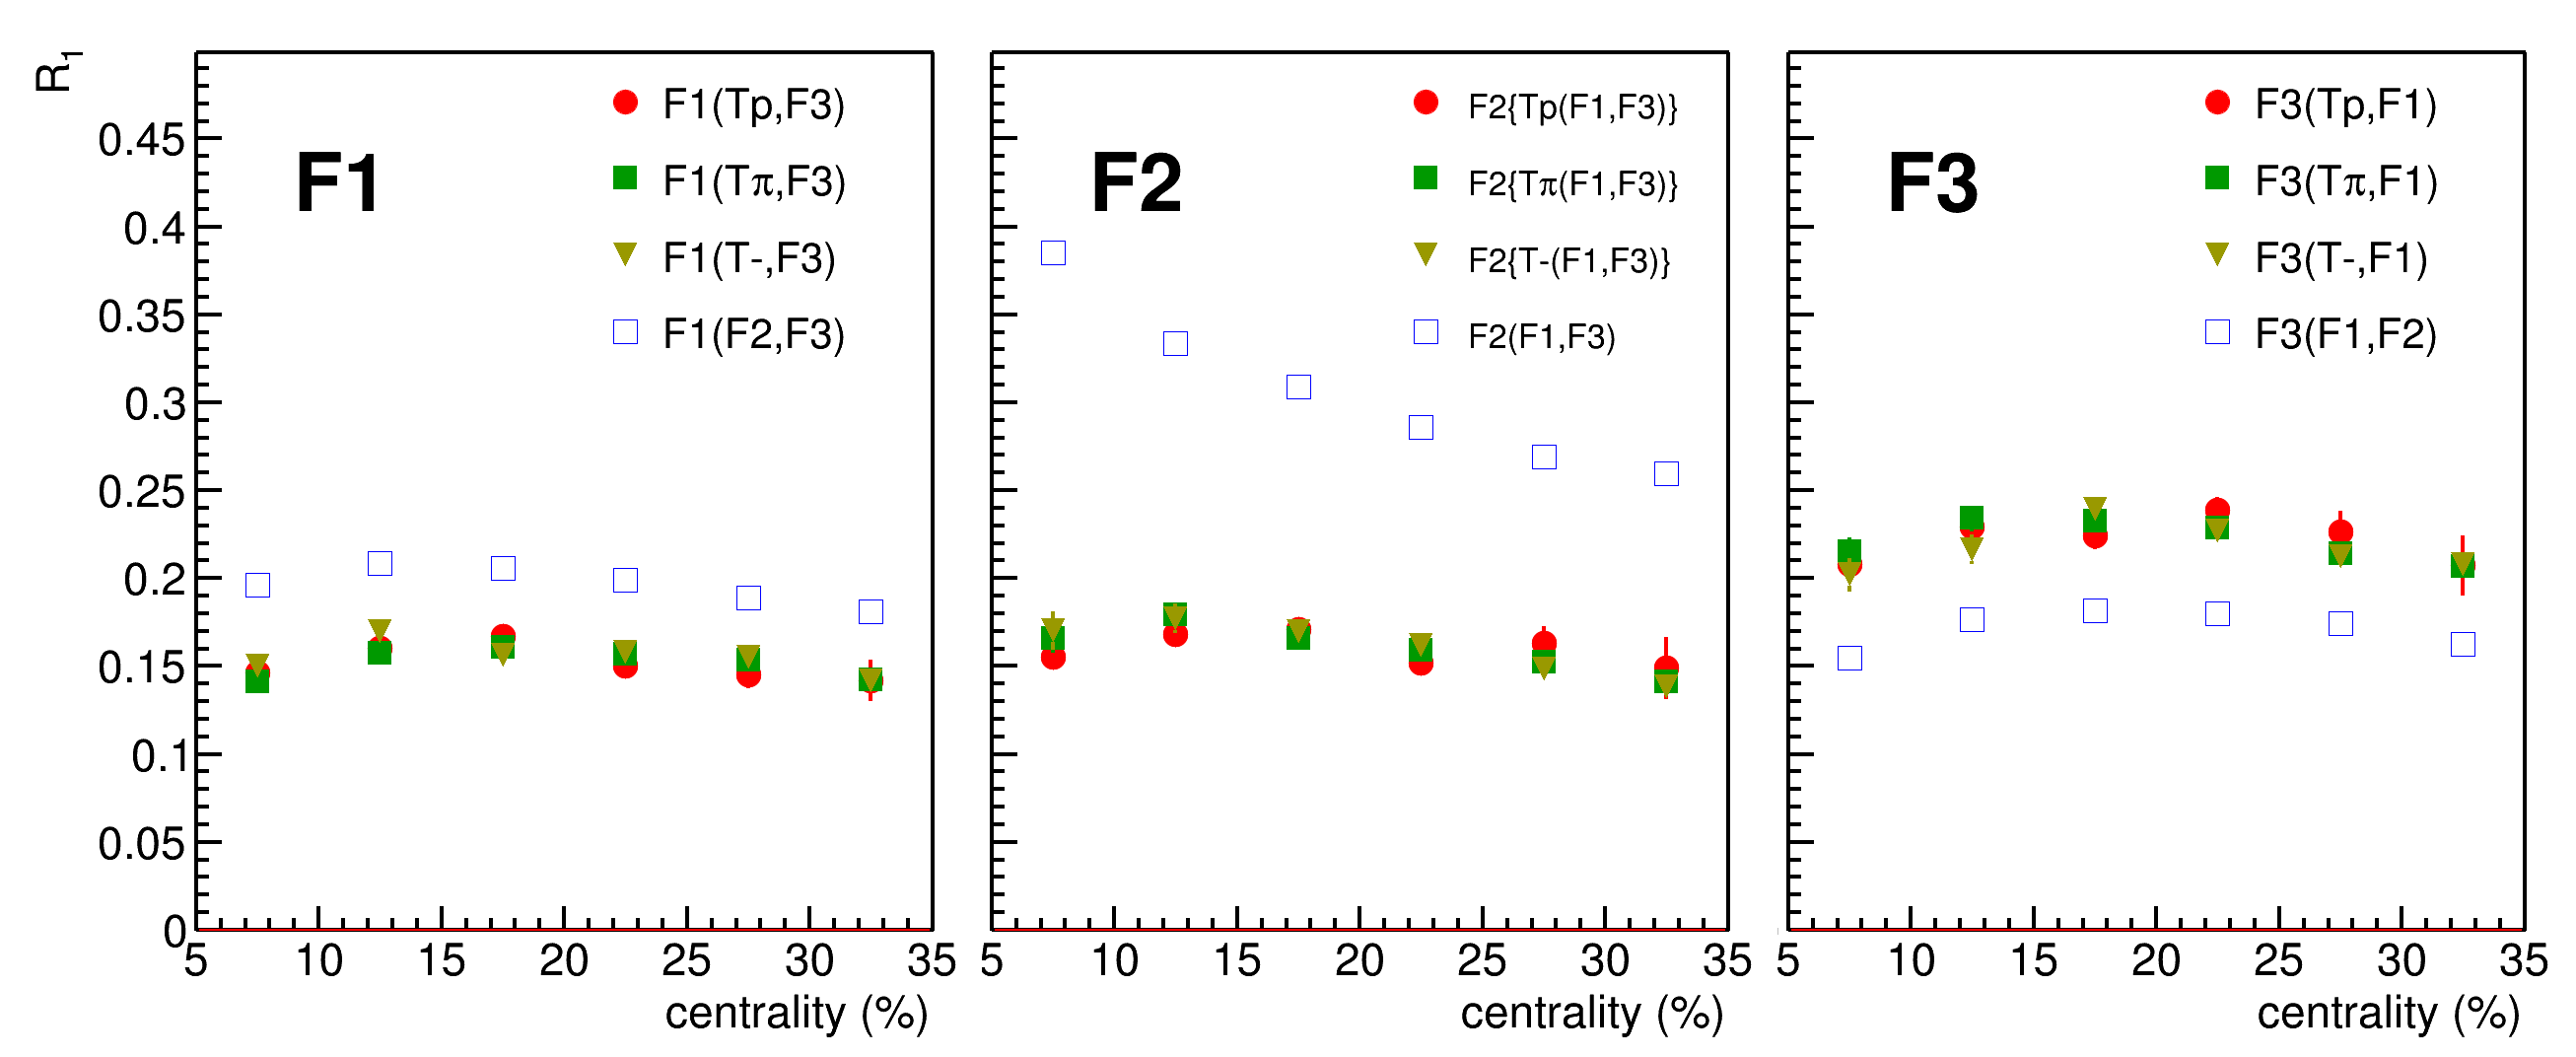
\includegraphics[width=0.95\linewidth]{images/R1_F123_combinations_centrality.png}
\caption{Разрешение плоскостей симметрии слева: $F1$, посередине: $F2$, справа: $F3$. Различные маркеры и цвета обозначают комбинации $Q_1$-векторов, использованных для расчета разрешения плоскости симметрии.}
\label{fig:bmn_combinations}
\end{center}
\end{figure}

\subsection{Исследование возможности измерения направленного и эллиптического потоков в эксперименте BM@N}

На рис.~\ref{fig:bmn_v1_v2} слева представлен направленный поток протонов, как функция быстроты в Монте-Карло моделировании столкновений $Xe+Cs$ из модели JAM. 
На рис.~\ref{fig:bmn_v1_v2} справа показан эллиптический поток протонов, как функция поперечного импульса в Монте-Карло моделировании столкновений $Xe+Cs$ из модели JAM. 
Разными цветами обозначена разная энергия столкновений. 
Линии обозначают $v_1$ и $v_2$ извлеченные напрямую из модели без реконструкции. 
Маркерами обозначены результаты анализа Монте-Карло моделирования отклика детектора.
Между данными извлеченными из модели и результатами анализа после реалистичной цепочки реконструкции наблюдается согласие в пределах статистической ошибки. 
%
\begin{figure}[ht]
\begin{center}
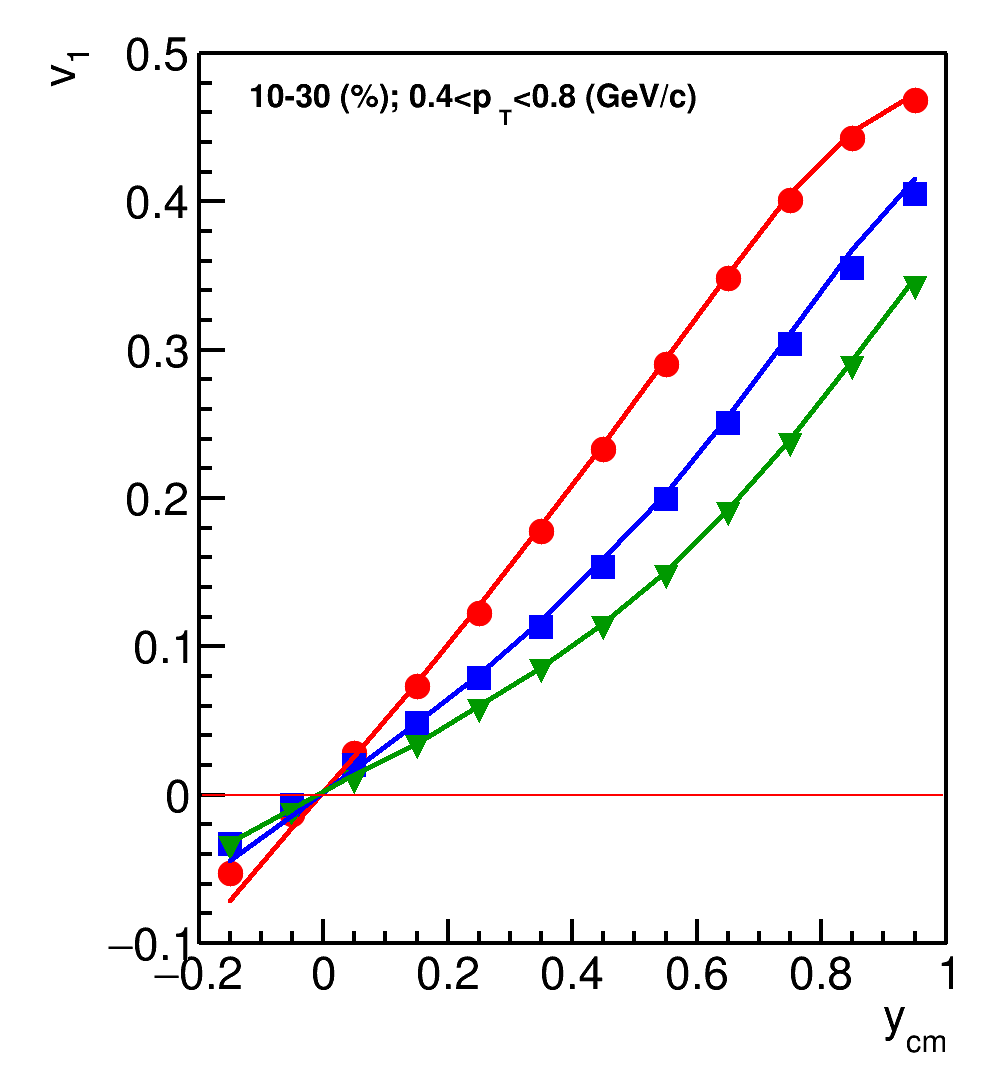
\includegraphics[width=0.45\linewidth]{images/v1_proton_tof_rapidity.png}
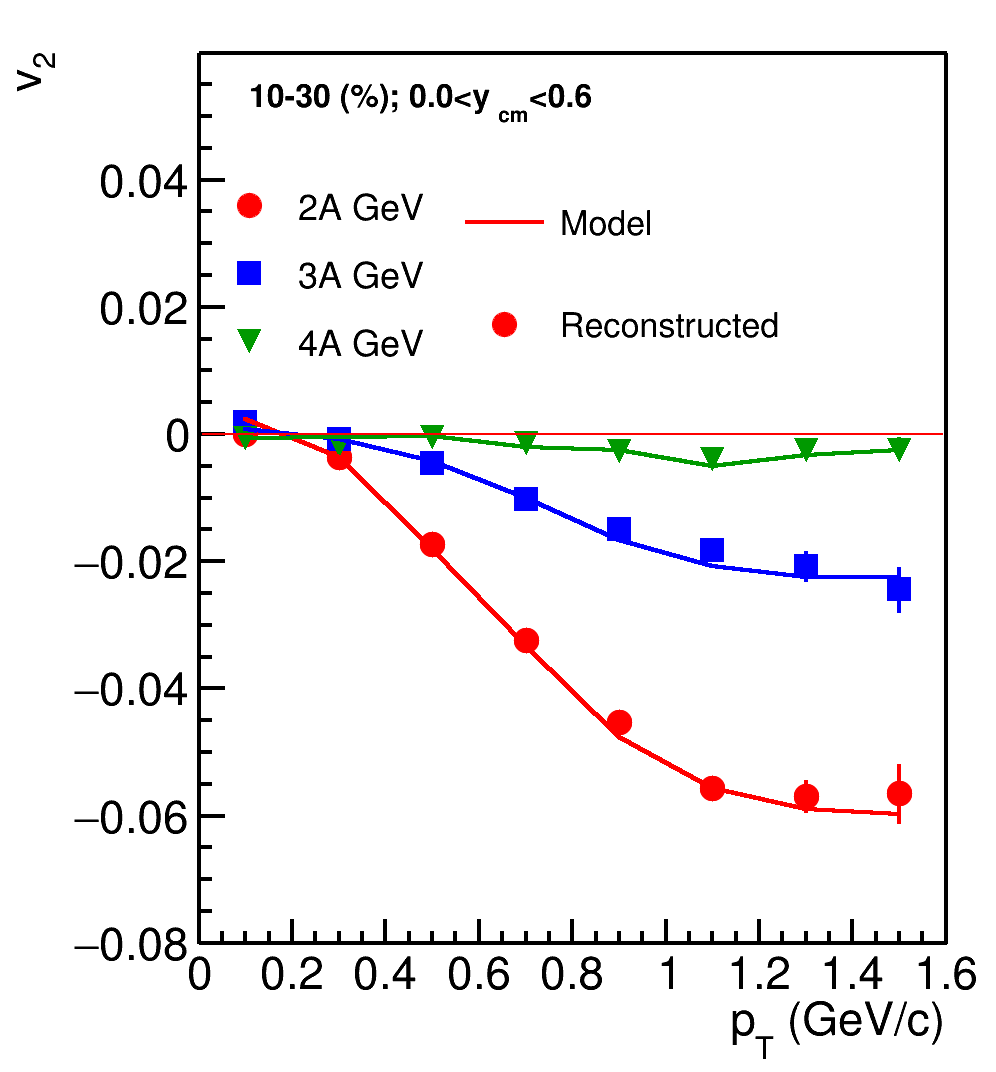
\includegraphics[width=0.45\linewidth]{images/v2_proton_tof_pT.png}
\caption{ 
    Направленный (слева) и эллиптический (справа) поток протонов как функция быстроты и поперечного импульса соответственно в Монте-Карло моделировании столкновений $Xe+Cs$ из модели JAM. Разными цветами обозначена разная энергия столкновений. Линии обозначают $v_1$ и $v_2$ извлеченные напрямую из модели без реконструкции. Маркерами обозначены результаты анализа Монте-Карло моделирования отклика детектора.
}
\label{fig:bmn_v1_v2}
\end{center}
\end{figure}